\documentclass[12pt]{article}

\usepackage[UTF8]{ctex}
\usepackage{appendix}
\usepackage{enumerate}
\usepackage{amsmath}
\usepackage{graphicx}
\usepackage{cite}
\usepackage{multirow}
\usepackage{geometry}
\usepackage[section]{placeins}
\usepackage[colorlinks,linkcolor=blue]{hyperref}
\title{\songti\zihao{1}电工电子综合实验\\(Ⅱ)\\\ \\\ \\  \heiti\zihao{2}多功能数字时钟\\ \ \\\  \\\ }
\author{\heiti\zihao{3}姓名:\underline{      许晓明      }\\ \\\heiti\zihao{3}学号:\underline{ 9161040G0734 }\\ \\\heiti\zihao{3}学院:\underline{ 电子工程与光电技术学院 }\\ \\\heiti\zihao{3}专业:\underline{  电子信息工程 }\\ \\\heiti\zihao{3}指导老师:\underline{ 丁淑艳 }\\ \\\heiti\zihao{3}2018年9月}
%\author{}
\date{}
\geometry{a4paper,scale=0.85}

\begin{document}%文档从这里开始。

\numberwithin{footnote}{section}
\renewcommand{\contentsname}{\centering 目录}
\renewcommand{\tablename}{表}
\renewcommand{\figurename}{图}
\renewcommand\refname{参考文献}
\renewcommand\appendix{\setcounter{secnumdepth}{0}}
\renewcommand\abstractname{摘要}


\maketitle
\newpage
\tableofcontents

\newpage
\section{设计内容简介}
本实验要求搭建一个多功能数字时钟的电路图,其具体要求如下:
\begin{enumerate}
\item 脉冲发生电路:为计时器提供秒脉冲、为报时电路提供驱动蜂鸣器的脉冲信号。
\item 计时电路:完成0分00秒~9分59秒的计时功能。
\item显示电路:通过数码管显示计时中的读数。
\item 清零电路:包括开机清零与手动清零功能。
\begin{enumerate}
\item 开机清零:开机自动清零功能。
\item 手动清零:在任意时刻,按动清零开关,可进行计时器清零。
\end{enumerate}
\item 校分电路:在任意时刻,拨动校分开关,可对分位进行快速校分。
\item 报时电路:使数字计时器从9分53秒开始报时,要求9分53秒、 9分55秒、9分57秒发低音(频率为1kHz),9分59秒发高音(频率为2kHz)。
\item 系统级联调试,将以上电路进行级联完成计时器的所有功能。
\end{enumerate}






\section{设计原理}
原理上,数字时钟是典型的数字电路,包括组合逻辑电路和时序电路等,由振荡器、分频器、计数器、显示器等几部分组成。\par首先由振荡器产生一定频率的信号,再由分频器选择输出所需要的1Hz标准频率进行计数。实验中我们使用石英晶体振荡器构成脉冲发生电路,用分频器和D触发器构成的二分频电路对脉冲进行分频,选取1Hz信号做秒个位时钟信号,同时选取2Hz信号用于校分电路,1KHz、2KHz用于蜂鸣器的低鸣与高鸣。\par主体计时电路主要有计时器、译码器及显示器构成。实验中使用一片CD4518对计时器的秒个位和分位进行计数,使用74LS161构成模六(六进制)计数器实现秒十位的计数。当低位计数器计满时,向高位产生一个脉冲信号,触发高位计数器计数。\par实验中由于所使用的计数器都有异步清零端,故可通过简单的电路就可以使电路具有开机清零功能和随时清零功能。\par设计报时电路时,通过加入一些组合逻辑门电路,可以实现要求的固定时刻蜂鸣器高低鸣。
\par同样,,借助组合逻辑门电路,加入校分电路,以便将分位及时跳到想要的时刻,也便于在检验电路时,蜂鸣器能尽早响起。\par这样,一个具有完整功能的数字计时器基本完成了。这个过程大致如图\ref{fig:zhentitu}所示。

\begin{figure}[h]
\centering
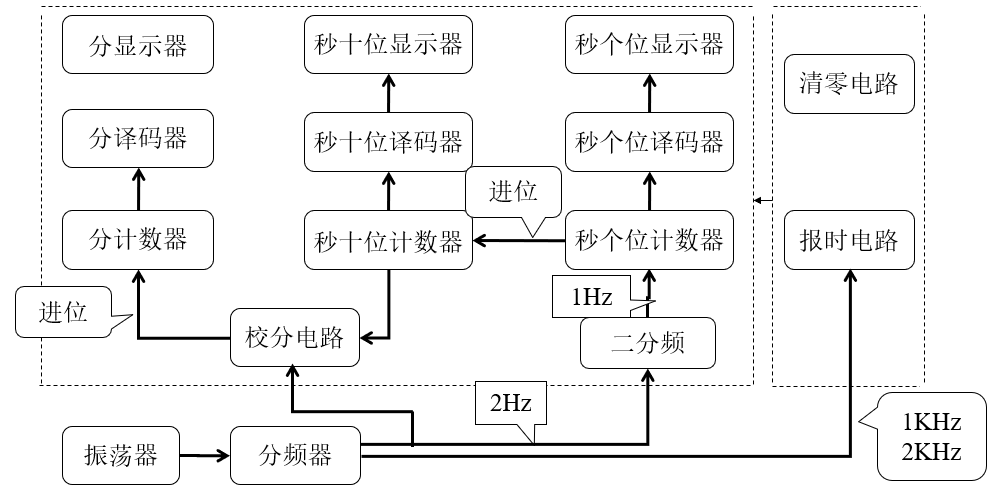
\includegraphics[width=\textwidth]{TIM20180920124456.png}
\caption{整体设计原理图}
  \label{fig:zhentitu}
\end{figure}
接下来,分别阐述各部分的设计原理及接线。
\subsection{脉冲发生电路}\label{begin}
首先搭建基于32768Hz的石英晶体多谐振荡器,再使用分频器CD4060(最高可实现214分频)进行分频。其中,最低频率端$Q_{14}$输出脉冲信号频率为2Hz,$Q_5$为1KHz,$Q_4$为2KHz。\par将74LS74\ D触发器的$\overline{Q}$ 端与D端相连,实现二分频,对2Hz频率进行分频以得到1Hz的信号,输出端为Q端。原理图如图\ref{fig:maichong}。
\begin{figure}[h]
\centering
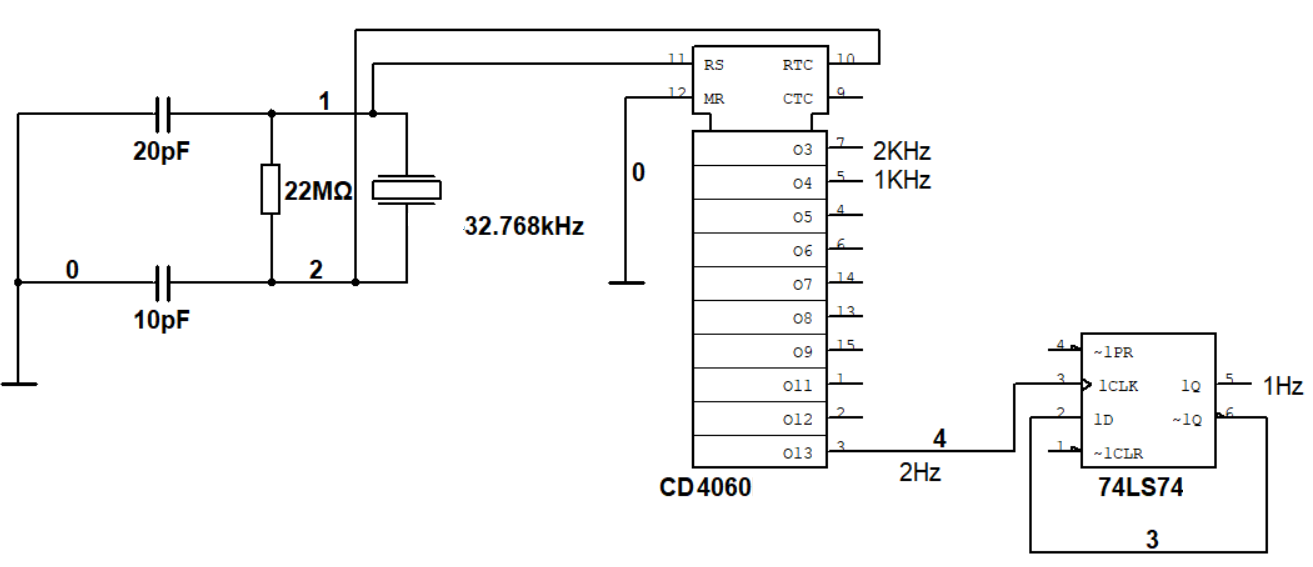
\includegraphics[width=\textwidth]{TIM20180923143758.png}
\caption{脉冲发生电路图}
  \label{fig:maichong}
\end{figure}
\par这一步所用器件有:32768Hz晶振$\times1$、CD4060$\times1$、74LS74$\times1$、22$M\Omega$电阻$\times1$、20pF电容$\times1$、10pF电容$\times1$、直流电源等。

\subsection{计时、显时电路}
在计时电路中,直接使用CD4518 BCD码计数器实现秒个位、分位的十进制计数功能,而秒十位计数器需要六进制计数器,于是将74LS161做成一个从0000$-$0101的模六计数器实现。\par在连接时,将脉冲发生电路产生的1Hz脉冲信号送入秒个位计数器(CD4518)的CP端,秒个位中的输出$1Q_4$通过一非门接入74LS161的时钟端作为时钟信号完成个位与十位的级联。做秒十位记数时,用反馈置位法,将$2Q_1$和$2Q_3$通过一与非门接入置数端同时数据输入端均接地,实现模六功能。将计数位2Q3作为驱动信号送入分计数器(CD4518)的EN端,同时CP端接地,此时CD4518下降沿有效,于是数字计数器整体的计数功能即可实现。\par而显示电路则采用三片CD4511显示译码器和三个七段共阴数码管,电路从0分00秒计到9分59秒,译码显示电路用三片四线七线译码器CD4511进行译码,而采用共阴极七段LED数码管进行循环显示。CD4511的输入接到相应计数器的输出,而它的输出端与数码管的相应端相连,数码管的共阴极通过$300\Omega$的电阻接地。\par完成后的电路见图\ref{fig:jishi}所示。
\par这一步所用器件有:CD4518$\times2$、74LS161$\times1$、74LS00$\times1$、CD4511$\times3$、CD4069$\times1$、300$\Omega$电阻$\times3$、LED数码显示管$\times3$、直流电源等。

\begin{figure}[h]
\centering
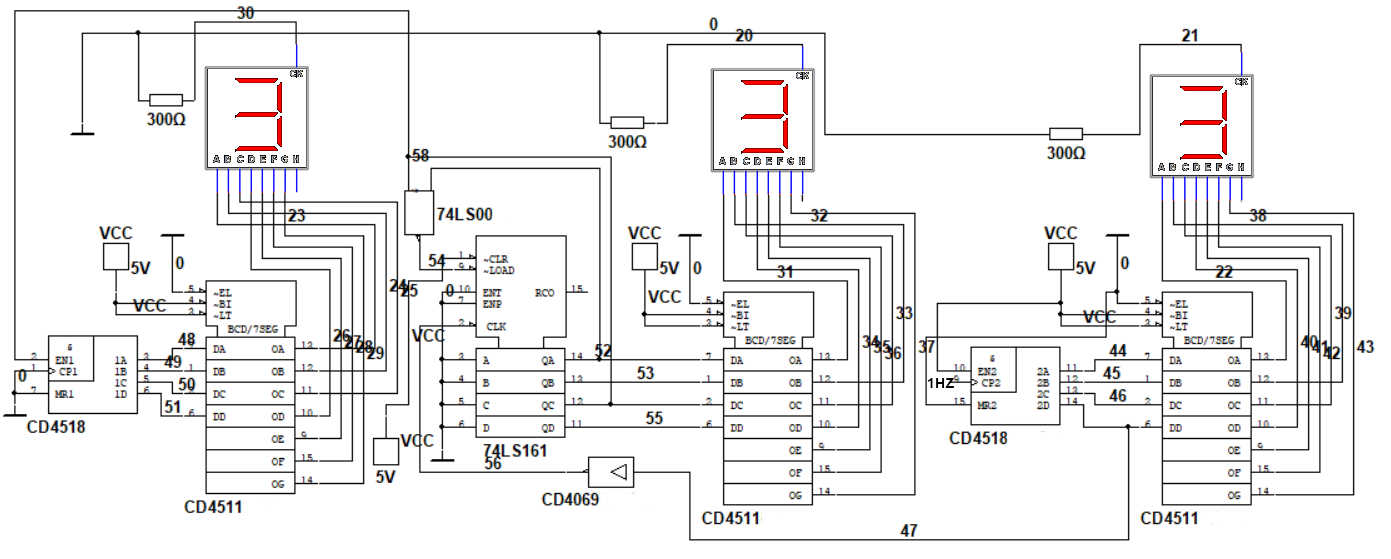
\includegraphics[width=\textwidth]{TIM20180923162121_1.png}
\caption{计时、显时电路图}
  \label{fig:jishi}
\end{figure}
\subsection{清零电路}
清零电路要实现两项功能:开机清零和任意时刻选择清零。其中秒个位和分位的清零端,即CD4518的管脚7和15(高电平有效)接在电路第一个非门之后,秒十位74LS161的清零端,即管脚1(低电平有效)则需接在第二个非门之后。\par刚开机时,由于电容上的电压不能突变,电容两端为低电平,经过第一个非门输出高电平,接到CD4518的管脚7和15,实现秒个位和分位的清零。再经过第二个非门输出低电平,接到74LS161的管脚1,实现秒十位的清零。按下开关后,电容被短路,第一个非门的输入端为低电平,两个非门的输出端分别为高电平和低电平,原理同上,实现控制清零功能 (异步清零)。\par完成后的电路见图\ref{fig:qingling}所示。
\par这一步所用器件有:CD4069$\times1$、10K$\Omega$电阻$\times1$、22uF电容$\times1$、直流电源。

\begin{figure}[h]
\centering
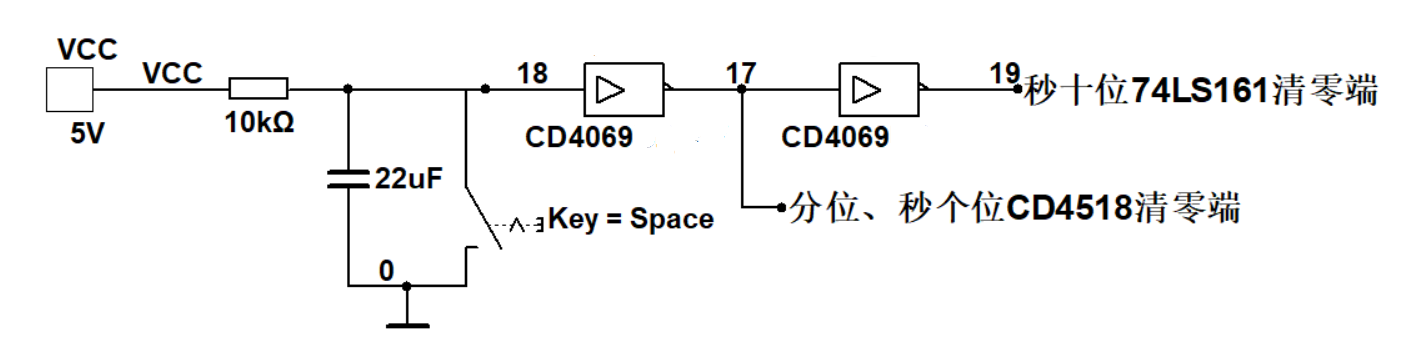
\includegraphics[width=\textwidth]{TIM20180922213402.png}
\caption{清零电路图}
  \label{fig:qingling}
\end{figure}
\subsection{校分电路}
校分电路是通过开关和逻辑门电路实现的。当校分电路开关断开时,电容正极为5V的高电位,于是接入2Hz信号的74LS00输出始终为1,计数器正常计数;而当开关闭合时,电容正极为0V的低电位,接入秒十进位信号的74LS00输出始终为1,秒个位和秒十位正常计数,但分计数器可以不受秒十计数器的进位信号的控制,分位将随2Hz信号进行快速校分。\par完成后的电路见图\ref{fig:jiaofen}所示。
\par这一步所用器件有:10$K\Omega$电阻$\times1$、22$\mu F$电容$\times1$、74LS00$\times1$、CD4069$\times1$、直流电源等。
\begin{figure}[h]
\centering
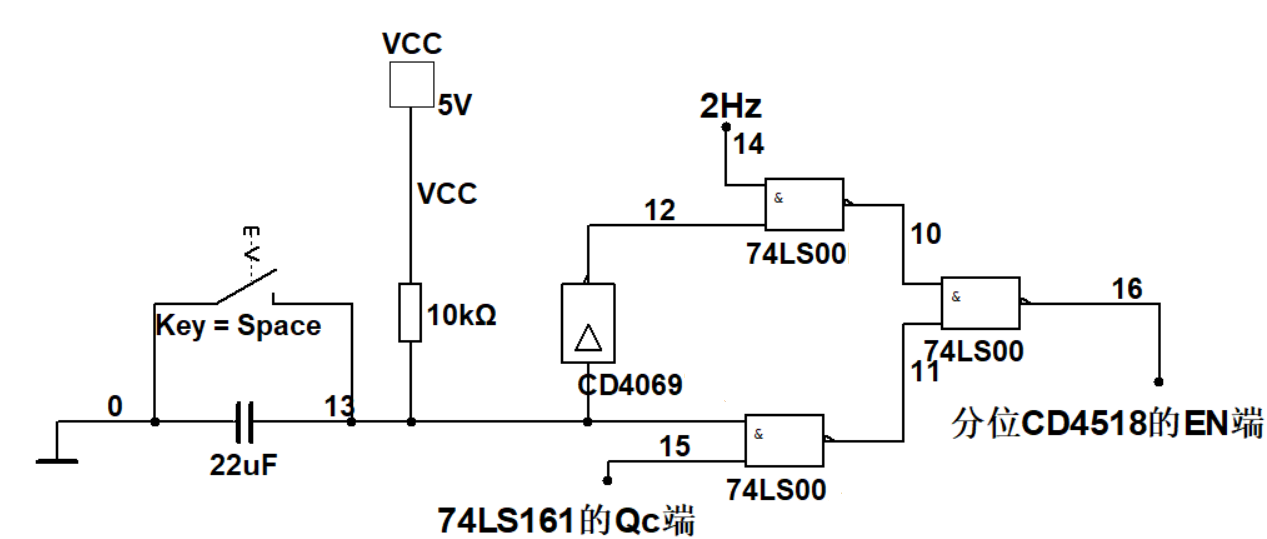
\includegraphics[width=\textwidth]{TIM20180922212603.png}
\caption{校分电路图}
  \label{fig:jiaofen}
\end{figure}

\subsection{报时电路}\label{end}
报时电路由逻辑门电路组成的。用需要报时的时刻所对应的计数器的输出作为触发信号来驱动蜂鸣器报时,因为需要在9分53秒、9分55秒、9分57秒各报出一个低音,在9分59秒报出一个高音,因此将各时刻各位对应的二进制码列表如表\ref{tab:time}。

\begin{table}[htbp]
  \centering
  \caption{需要报时的时刻及其二进制码}
    \begin{tabular}{cccc}
    \hline
    时间(DEC) & 分位(BIN) & 秒十位(BIN) & 秒个位(BIN) \\
    \hline
    9:53:00 & 1001 & 0101 & 0011 \\
    9:55:00 & 1001 & 0101 & 0101 \\
    9:57:00 & 1001 & 0101 & 0111 \\
    9:59:00 & 1001 & 0101 & 1001 \\
    \hline
    \end{tabular}%
  \label{tab:time}%
\end{table}%
\begin{enumerate}
\item 将秒个位的3(0011)、5(0101)、7(0111)取或,通过卡诺图的化简可知应该从秒个位取$1Q_A\cap(1Q_B+1Q_C)$
\item 将1中所得结果和分位的9(1001)取与,再和秒十位的5(0101)取与,所得的结果和1KHz的信号取与,就可得到在9分53秒、9分553秒、9分57秒报出低音的驱动信号。
\item  将分位的9(1001)和秒十位的5(0101)取与,再和秒个位的9(1001)取与,再和2KHz的信号取与,就得到在9分59秒报出高音的驱动信号。
\item 将2和3中得到的信号取或,就可以得到最终的报时驱动信号,其原理图见图\ref{fig:baoshi}。
\end{enumerate}
这一步所用器件有:74LS21$\times2$、74LS32$\times1$、蜂鸣器$\times1$、直流电源等。
\begin{figure}[h]
\centering
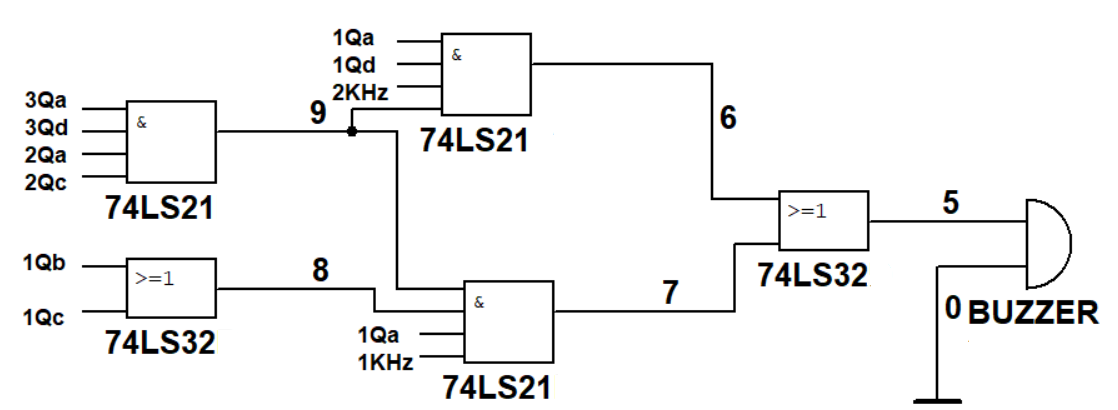
\includegraphics[width=\textwidth]{TIM20180922134052.png}
\caption{报时电路图}
  \label{fig:baoshi}
\end{figure}

\section{实验部分故障情况及排除方法}
\begin{enumerate}
\item 遇到问题:脉冲发生电路无效。\\解决方案:多次检查,发现是晶振接触不良,重新插好晶振后可以工作。
\item 遇到问题:清零电路无效。\\解决方案:线路接触不良,重新布线后可以工作。
\item 遇到问题:清零电路无法开机清零。\\解决方案:关机、开机时间间隔太短,电容未完全放电。关机一段时间后通电,发现清零电路事实上可以工作。
\item 遇到问题:接入校分电路后发现电路无效。\\解决方案:多次检查元件间的连线无果,后经过研究,发现是校分电路的电阻阻值过大,充电时间过长。更换电阻后电路正常工作。
\item 遇到问题:报时电路只有59秒时有声音,53、55、57秒无效。\\解决方案:秒个为输出端连线出错,多次检查元件间的连线,正确布线后可以工作。
\end{enumerate}

\section{实验体会}
\subsection{针对电路连接的体会}
电路连接过程中要注意以下几点:
\begin{enumerate}
\item 由于实验中的芯片对电压比较敏感,直流电源统一使用5V,且要用万用表测量,确定直流输出范围在$4.9-5.1V$后方可使用。
\item 用指针万用表检测1Hz信号时,将万用表调到10V直流档位,黑表笔接地,红表笔接CD4518的CP端,万用表数值发生跳动,且变化的频率约为1次/秒,则说明正常输出。
\item 由于电阻有限,限流时,数码管接地端直接串联300欧姆电阻即可,而不是在a至g端分别串接。而由于共用电阻,在显示时,会出现亮起的LED管越多,显示越暗的情况,是正常现象。
\item 所有功能管脚均不能悬空,因为悬空会使电路输入不稳定或接触不良等。
\item 清零电路接入前,需要使秒个位、秒十位、分位的清零端无效;而在接入清零电路,则需要根据清零电路原理分别接入清零信号,同时去除原来的清零端无效状态。
\item 校分电路接入时,需要将原本来自秒十位的进位信号(分位的计数端)根据校分电路的原理,改接成校分信号的输出端,否则,校分电路将无法正常使用。
\item 所有芯片在安装时,要注意电源、电源地是否有效连接。由于在电路图中,这一点无法体现,可能会被遗漏。
\item 集成器件接线时,应该注意导线不宜太长,最好贴近底板器件周围走线;切忌跨越上空成网状;布线、布局应合理、整齐、美观;开关的断开与闭合用导线代替。
\item 在排布芯片时,最好有所设计,避免因前期芯片排布的不合理造成后期大量飞线的情况。
\end{enumerate}
\subsection{针对实验过程的体会}
电工电子综合实验,不仅对设计能力提出了一定要求,也在动手能力方面有一定的要求。在已知电路图的情况下,能否正确、快速的连接成功,也成为考验耐心和细心的一项难题。事实上,在连接电路时,由于前期准备不足,又没有较为冷静的思考,致使完成的速度不尽如人意。\par今后,在解决问题时,希望自己能够做到:事前有准备、处事有条理、遇事有头脑。不眼高手低,急于求成,也不妄自菲薄,缺少信心。


\appendix
\section{附录}
\begin{thebibliography}{15}\zihao{5}\addcontentsline{toc}{subsection}{参考文献}
\bibitem{}王建新,姜萍,等.电子线路实践教程[M]. 北京:科学出版社, 2003.
\bibitem{pingguo}蒋立平.数字逻辑电路与系统设计(第2版)[M]. 北京:电子工业出版社,2013.
\end{thebibliography}
\subsection{电路总图}
将\ref{begin}$-$\ref{end}所述的电路整合在一起,即可得到完整电路图如图\ref{fig:zong}。
\begin{figure}[h]
\centering
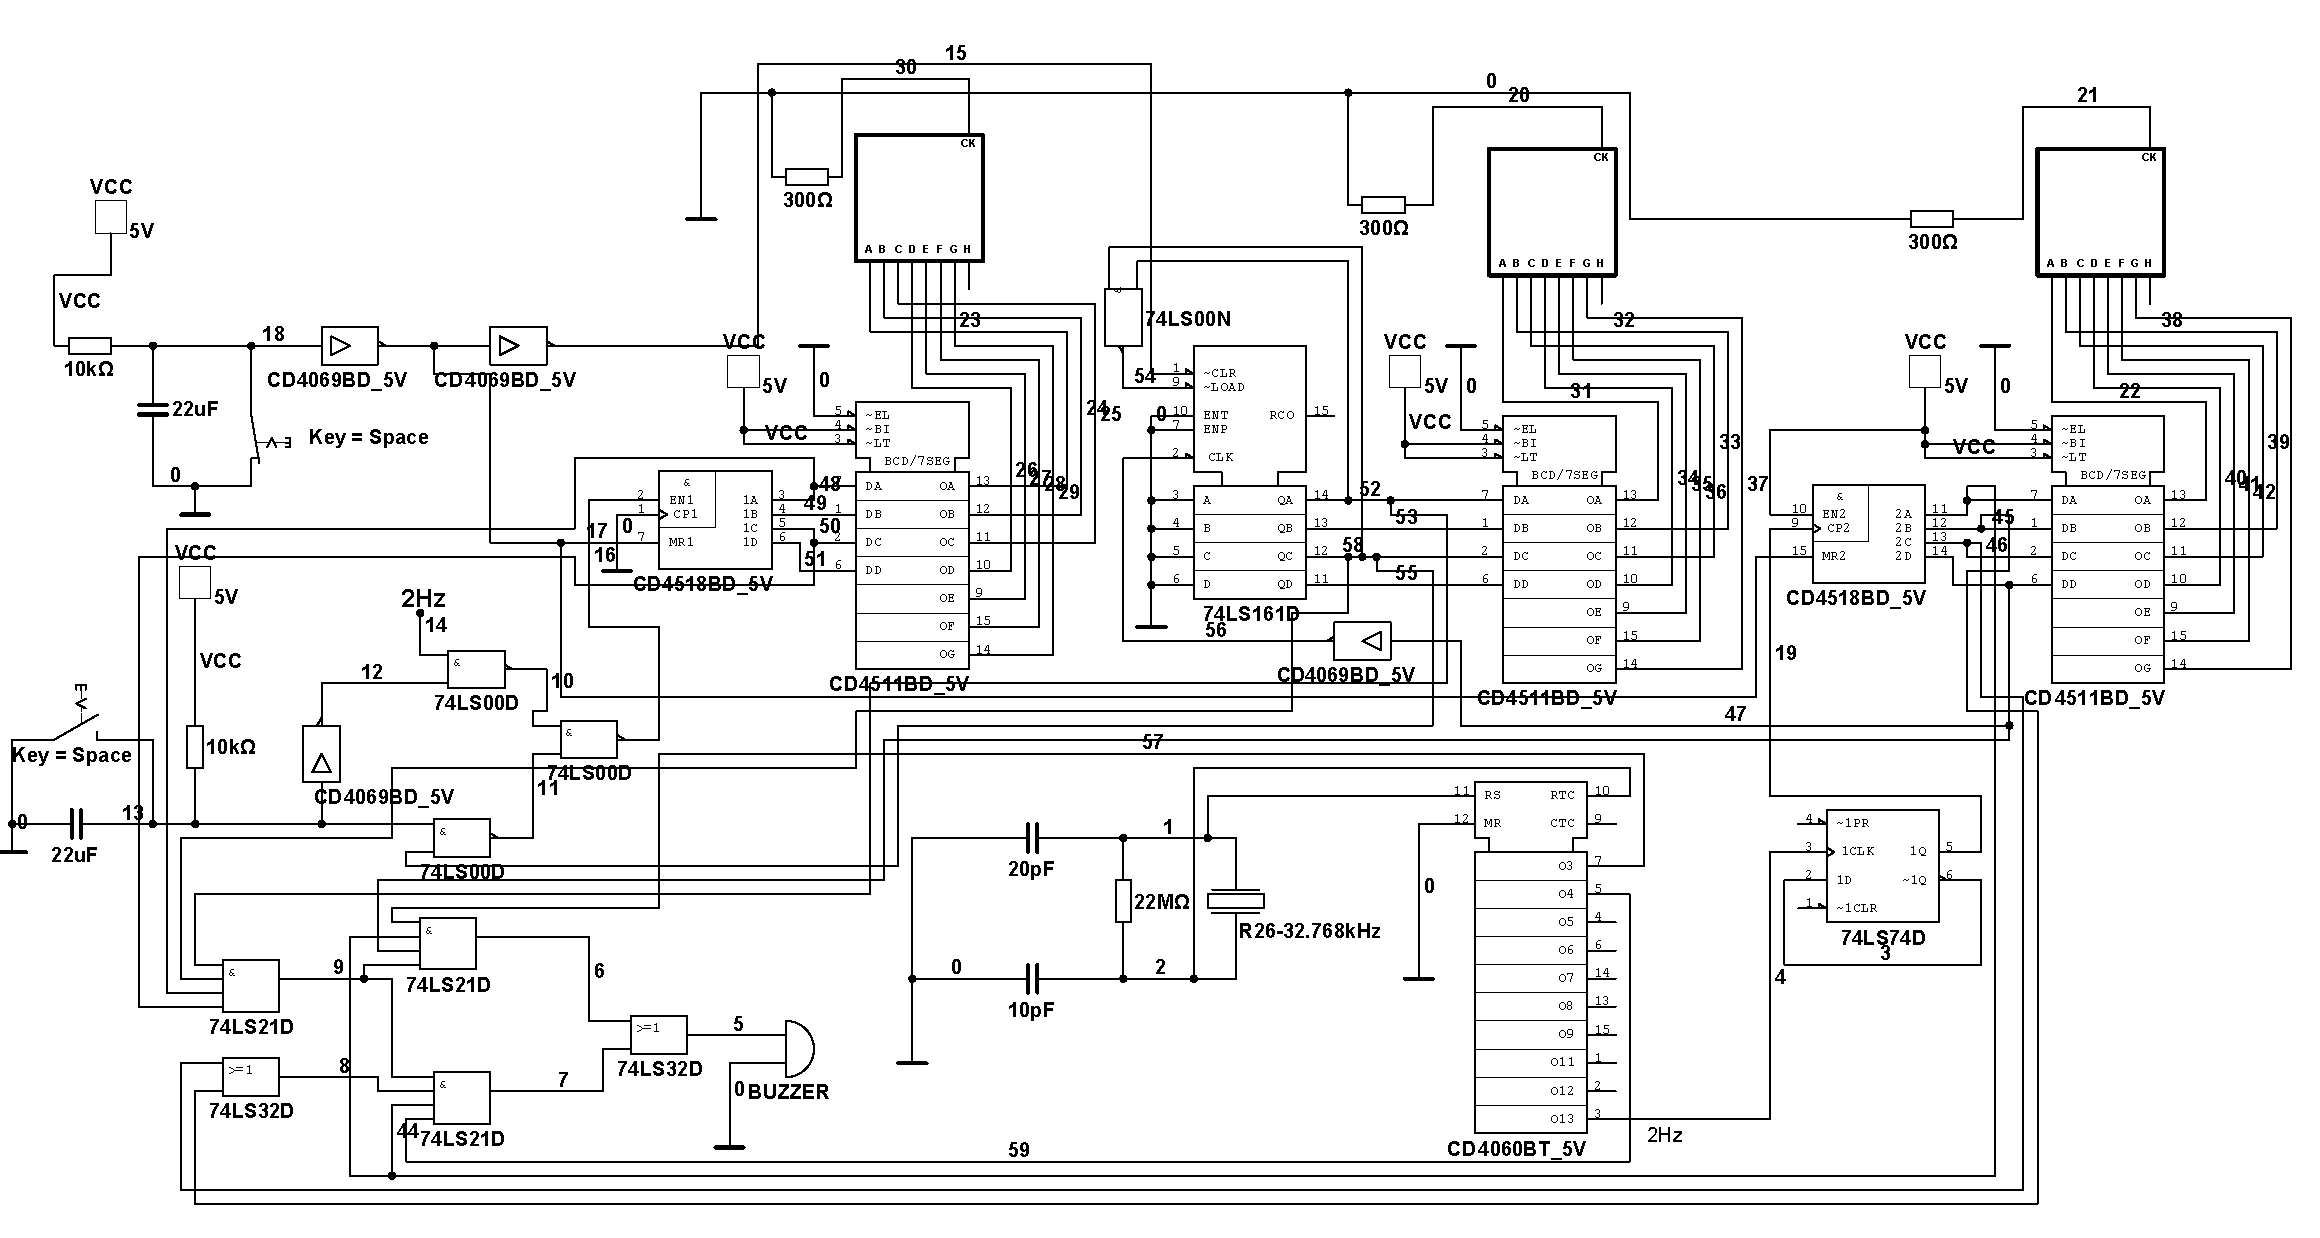
\includegraphics[width=\textwidth]{zong.png}
\caption{电路总图}
  \label{fig:zong}
\end{figure}
\subsection{实验工具及元器件清单}
实验用到的工具有:电源、镊子、剥线钳等。

元器件清单见表\ref{tab:addlabel1}。
\begin{table}[h]
  \centering
  \caption{元器件清单}
    \begin{tabular}{ccc}
    \hline
    名称 & 型号 & 数量 \\
        \hline
    LED数码管 & 共阴 & 3 \\
    译码器 & CD4511 & 3 \\
    BCD码计数器 & CD4518 & 2 \\
    4位二进制计数器 & 74LS161 & 1 \\
    分频器 & CD4060 & 1 \\
    D触发器 & 74LS74 & 1 \\
    非门 & CD4069 & 1 \\
    二输入与非门 & 74LS00 & 1 \\
    四输入与门 & 74LS21 & 2 \\
    二输入或门 & 74LS32 & 1 \\
    晶振 & 32768Hz & 1 \\
    蜂鸣器 &/& 1 \\
    \hline
    \multirow{3}*{电容}&10p	&1\\
    ~ & 20p & 1  \\
    ~&22$\mu$&2\\
    \hline
     \multirow{3}*{电阻} &300 & 3 \\
     ~  & 10k & 2 \\
       ~& 22M & 1 \\
        \hline
    \end{tabular}%
  \label{tab:addlabel1}%
\end{table}%


\subsection{芯片管脚排列图、逻辑图与功能表}
\subsubsection{管脚排布图}
各实验芯片的管脚排布图参见图\ref{fig:guanjiao}
\begin{figure}[h]
\centering
\begin{tabular}{ccc}
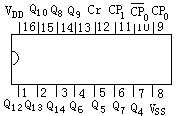
\includegraphics[width=0.3\textwidth]{CD4060.png}&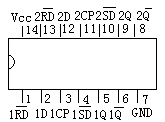
\includegraphics[width=0.3\textwidth]{7474.png}&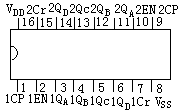
\includegraphics[width=0.3\textwidth]{CD4518.png}\\
CD4060&74LS74&CD4518\\
&&\\
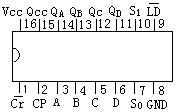
\includegraphics[width=0.3\textwidth]{74161.png}&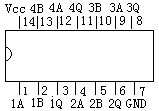
\includegraphics[width=0.3\textwidth]{7400.png}&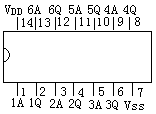
\includegraphics[width=0.3\textwidth]{CD4069.png}\\
74LS161&74LS00&CD4069\\
&&\\
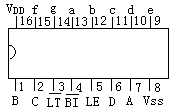
\includegraphics[width=0.3\textwidth]{CD4511.png}&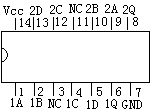
\includegraphics[width=0.3\textwidth]{7421.png}&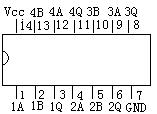
\includegraphics[width=0.3\textwidth]{7432.png}\\
CD4511&74LS21&74LS32\\
&&\\
 & 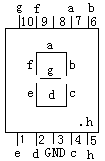
\includegraphics[width=0.18\textwidth]{LED.png} & \\
 &LED数码管&\\
  \end{tabular}
\caption{芯片管脚排布图}
  \label{fig:guanjiao}
\end{figure}
\subsubsection{芯片逻辑图}
各芯片在multisim中的逻辑图见图\ref{fig:luoji}所示。
\begin{figure}[h]
\centering
\begin{tabular}{ccccc}
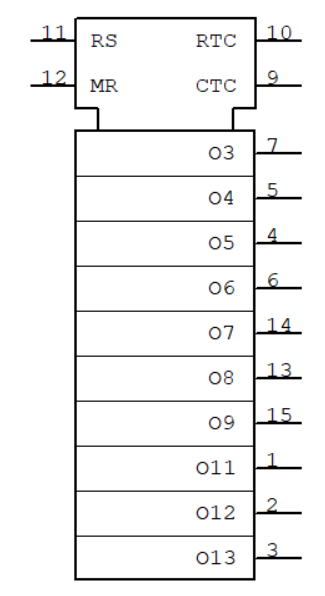
\includegraphics[width=0.18\textwidth]{TIM20180923144839.png}&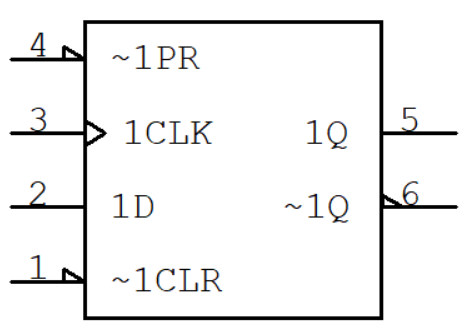
\includegraphics[width=0.18\textwidth]{TIM20180923145234.png}&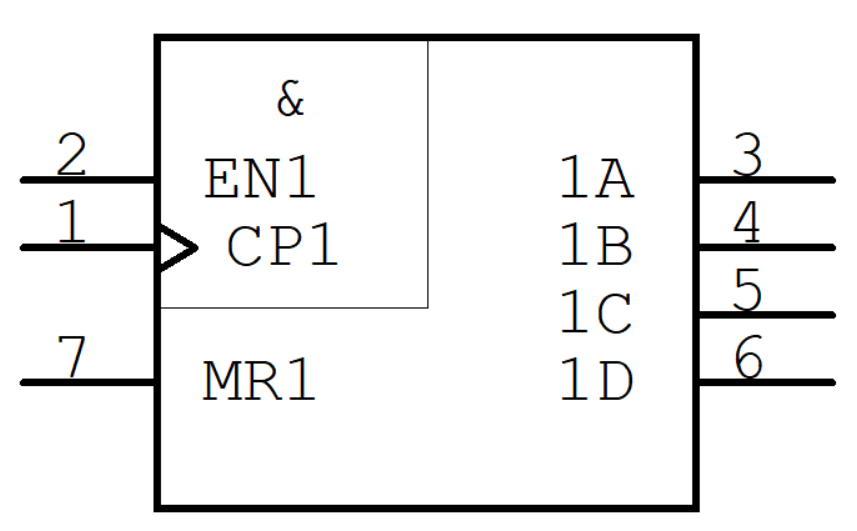
\includegraphics[width=0.18\textwidth]{TIM20180923145642.png}&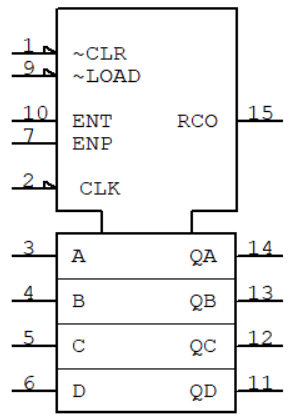
\includegraphics[width=0.18\textwidth]{TIM20180923150127.png}&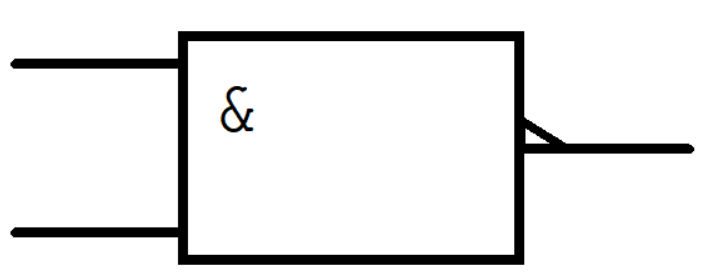
\includegraphics[width=0.18\textwidth]{TIM20180923150834.png}\\
CD4060&74LS74&CD4518&74LS161&74LS00\\
\\
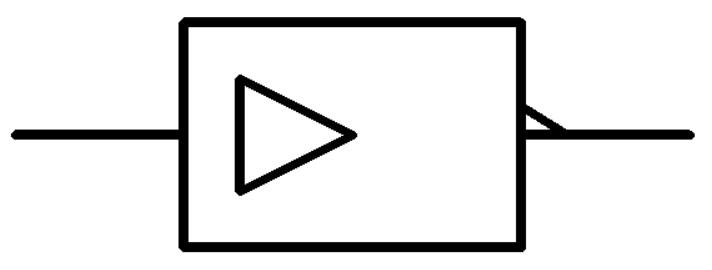
\includegraphics[width=0.18\textwidth]{TIM20180923151008.png}&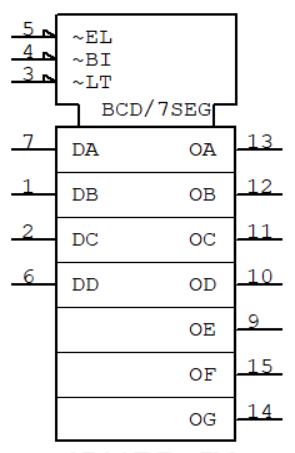
\includegraphics[width=0.18\textwidth]{TIM20180923151644.png}&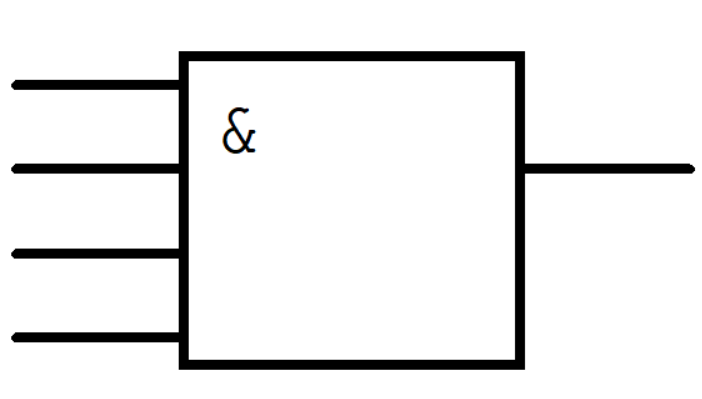
\includegraphics[width=0.18\textwidth]{TIM20180923151902.png}&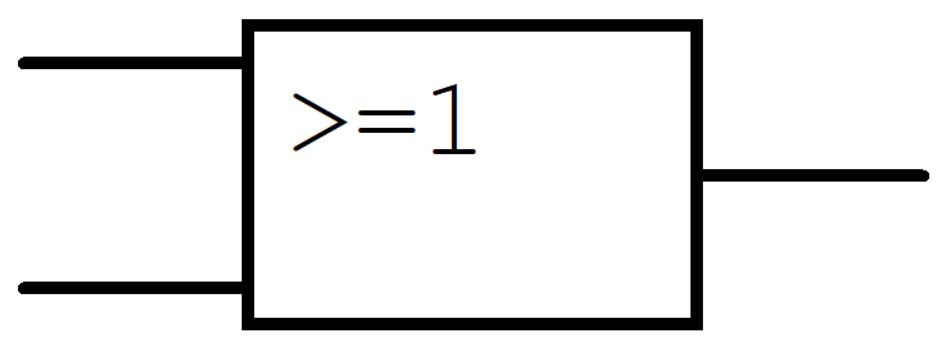
\includegraphics[width=0.18\textwidth]{TIM20180923152133.png}&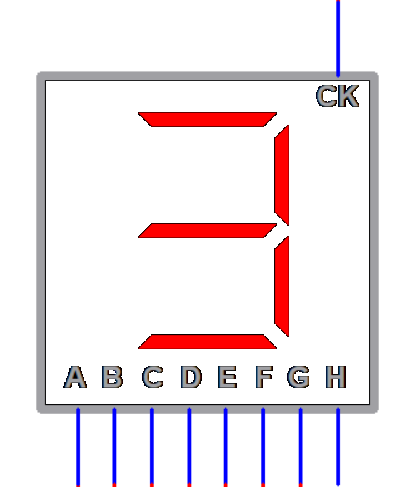
\includegraphics[width=0.18\textwidth]{TIM20180923152329.png}\\
CD4069&CD4511&74LS21&74LS32&LED数码管\\
  \end{tabular}
\caption{芯片在multisim中的逻辑图}
  \label{fig:luoji}
\end{figure}
\subsubsection{逻辑功能表}
各元器件的逻辑功能表参见表\ref{tab:7474}$-$\ref{tab:7432}。
% Table generated by Excel2LaTeX from sheet 'Sheet3'
\begin{table}[h]
  \centering
  \caption{74LS74逻辑功能表}
    \begin{tabular}{c|cccc|cc}
    \hline
  \multirow{2}*{功能}& \multicolumn{4}{c}{输入}  & \multicolumn{2}{|c}{输出}   \\
       & $CP$ &$ \overline{R_D}$ & $\overline{S_D}$ & $D$  & $Q_N$ & $\overline{Q_{N-1}}$ \\
        \hline
    清零 & $\times$  & 0  & 1  &$\times$  & 0  & 1 \\
    置\ 1& $\times$ & 1  & 0  & $\times$  & 1  & 0 \\
    送\ 0 & $\uparrow$  & 1  & 1  & 0  & 0  & 1 \\
    送\ 1 &  $\uparrow$   & 1  & 1  & 1  & 1  & 0 \\
    保持 & 0  & 1  & 1  & $\times$  &  \multicolumn{2}{c}{保持}\\
    不允许 & $\times$  & 0  & 0  & $\times$  &  \multicolumn{2}{c}{不确定} \\
     \hline
    \end{tabular}%
  \label{tab:7474}%
\end{table}%
% Table generated by Excel2LaTeX from sheet '4518'
\begin{table}[h]
  \centering
  \caption{CD4518逻辑功能表}
    \begin{tabular}{c|ccc|cccc}
      \hline
  \multirow{2}*{功能}& \multicolumn{3}{c|}{输入} &\multicolumn{4}{c}{ 输出}  \\
       & $Cr$ & $CP$ & $EN$ & $Q_D$ &$ Q_C$ & $Q_B$ & $Q_A$ \\
         \hline
    清零 & 1  &$ \times$ & $\times$ & 0  & 0  & 0  & 0 \\
    计数 & 0  &$ \uparrow$ & 1  &\multicolumn{4}{c}{  BCD码加法记数} \\
    保持 & 0  &$ \times$ & 0  & \multicolumn{4}{c}{ 保持}\\
    计数 & 0  & 0  & $\downarrow$ & \multicolumn{4}{c}{ BCD码加法记数} \\
    保持 & 0  & 1  & $\times$& \multicolumn{4}{c}{ 保持}  \\
      \hline
    \end{tabular}%
  \label{tab:4518}%
\end{table}%

% Table generated by Excel2LaTeX from sheet '74161'
\begin{table}[h]
  \centering
  \caption{74LS161逻辑功能表}
    \begin{tabular}{c|ccccccccc|ccccc}
      \hline
    \multirow{2}*{功能}& \multicolumn{9}{c}{输入} &\multicolumn{5}{|c}{ 输出}\\
       & $CP$ & $\overline{Cr} $& $\overline{LD} $& $S_0$ & $S_1$ &$ D$  &$ C$  &$ B$  & $A $ & $Q_D$ & $Q_C$ &$ Q_B$ & $Q_A$ & $Q_{CC}$ \\
         \hline
    清零 & $\times$ & 0  &$ \times$ & $\times$ & $\times$ & $\times$ & $\times$ & $\times$ & $\times$ & 0  & 0  & 0  & 0  & 0 \\
    送数 & $\uparrow$ & 1  & 0  & $\times$ & $\times$ & d  & c  & b  & a  & d  & c  & b  & a  & 0-1 \\
    记数 & $\uparrow $& 1  & 1  & 1  & 1  &$ \times$ & $\times$ & $\times$ & $\times$ & \multicolumn{5}{c}{二进制加法记数}\\
    保持 & $\times$ & 1  & 1  & 0  &$ \times$ &$ \times$ & $\times$ &$ \times$ & $\times$ &  \multicolumn{5}{c}{不变}  \\
    保持 & $\times$ & 1  & 1  &$ \times$ & 0  &$ \times $& $\times$ &$ \times $&$ \times$ &  \multicolumn{5}{c}{不变} \\
      \hline
    \end{tabular}%
  \label{tab74161}%
\end{table}%
% Table generated by Excel2LaTeX from sheet '7400'
\begin{table}[h]
  \centering
  \caption{74LS00逻辑功能表}
    \begin{tabular}{cc|c}
    \hline
     \multicolumn{2}{c|}{输入}& 输出 \\
    A  & B  & Q \\
    \hline
    0  & 0  & 1 \\
    0  & 1  & 1 \\
    1  & 0  & 1 \\
    1  & 1  & 0 \\
    \hline
    \end{tabular}%
  \label{tab:7400}%
\end{table}%
% Table generated by Excel2LaTeX from sheet '4069'

\begin{table}[h]
  \centering
  \caption{CD4096逻辑功能表}
    \begin{tabular}{c|c}
     \hline
    输入 & 输出 \\
     \hline
    0  & 1 \\
    1  & 0 \\
     \hline
    \end{tabular}%
  \label{tab:4096}%
\end{table}%

% Table generated by Excel2LaTeX from sheet 'CD4511'
\begin{table}[h]
  \centering
  \caption{CD4511逻辑功能表}
    \begin{tabular}{c|ccccccc|ccccccc|c}
     \hline
    \multirow{2}*{功能} &  \multicolumn{7}{c|}{输入} &  \multicolumn{7}{c|}{输出} & \multirow{2}*{字符} \\
       & $\overline{LT}$ & $\overline{BI}$ & $LE$ & $D$ & $C$ & $B$ & $A$ & g  & f  & e  & d  & c  & b  & a  &  \\
        \hline
    测灯 & 0  & $\times$ & $\times$ & $\times$ & $\times$ & $\times$ & $\times$ & 1  & 1  & 1  & 1  & 1  & 1  & 1  & 8 \\
    灭零 & 1  & 0  & $\times$ & 0  & 0  & 0  & 0  & 0  & 0  & 0  & 0  & 0  & 0  & 0  & 消隐 \\
    锁存 & 1  & 1  & 1  & $\times$ & $\times$ & $\times$ & $\times$ & \multicolumn{8}{c}{显示$LE=0\rightarrow1$时数据} \\
    \multirow{10}*{译码} & 1  & 1  & 0  & 0  & 0  & 0  & 0  & 0  & 1  & 1  & 1  & 1  & 1  & 1  & 0 \\
       & 1  & 1  & 0  & 0  & 0  & 0  & 1  & 0  & 0  & 0  & 0  & 1  & 1  & 0  & 1 \\
       & 1  & 1  & 0  & 0  & 0  & 1  & 0  & 1  & 0  & 1  & 1  & 0  & 1  & 1  & 2 \\
       & 1  & 1  & 0  & 0  & 0  & 1  & 1  & 1  & 0  & 0  & 1  & 1  & 1  & 1  & 3 \\
       & 1  & 1  & 0  & 0  & 1  & 0  & 0  & 1  & 1  & 0  & 0  & 1  & 1  & 0  & 4 \\
       & 1  & 1  & 0  & 0  & 1  & 0  & 1  & 1  & 1  & 0  & 1  & 1  & 0  & 1  & 5 \\
       & 1  & 1  & 0  & 0  & 1  & 1  & 0  & 1  & 1  & 1  & 1  & 1  & 0  & 0  & 6 \\
       & 1  & 1  & 0  & 0  & 1  & 1  & 1  & 0  & 0  & 0  & 0  & 1  & 1  & 1  & 7 \\
       & 1  & 1  & 0  & 1  & 0  & 0  & 0  & 1  & 1  & 1  & 1  & 1  & 1  & 1  & 8 \\
       & 1  & 1  & 0  & 1  & 0  & 0  & 1  & 1  & 1  & 0  & 0  & 1  & 1  & 1  & 9 \\
        \hline
    \end{tabular}%
  \label{tab:4511}%
\end{table}%

% Table generated by Excel2LaTeX from sheet '7421'
\begin{table}[h]
  \centering
  \caption{74LS21逻辑功能表}
    \begin{tabular}{cccc|c}
     \hline
      \multicolumn{4}{c|}{输入}& 输出 \\
    $A$  &$ B$  &$ C$  &$ D$  &$ Q$ \\
     \hline
    0  & $\times$ & $\times$ & $\times$ & 0 \\
    $\times$ & 0  & $\times$ & $\times$ & 0 \\
    $\times$ & $\times$ & 0  & $\times$ & 0 \\
    $\times$ & $\times$ & $\times$ & 0  & 0 \\
    1  & 1  & 1  & 1  & 1 \\
     \hline
    \end{tabular}%
  \label{tab7421}%
\end{table}%

% Table generated by Excel2LaTeX from sheet '7432'
\begin{table}[h]
  \centering
  \caption{74LS32逻辑功能表}
    \begin{tabular}{cc|c}
     \hline
     \multicolumn{2}{c|}{输入}& 输出 \\
    $A$ & $B$ & $Q$ \\
     \hline
    0  & 0  & 0 \\
    0  & 1  & 1 \\
    1  & 0  & 1 \\
    1  & 1  & 1 \\
     \hline
    \end{tabular}%
  \label{tab:7432}%
\end{table}%

\end{document}
